\documentclass[letter]{report}
\usepackage{amsthm,amsmath,amssymb,bm,epic,geometry, graphicx, subfigure, epsfig} 
\oddsidemargin -0.25in 
\textwidth 6.5in 

%\newcommand {\linespace}{\renewcommand{\baselinestretch}{2}}
%\linespace
\newtheorem{thm}{Theorem}[section]
\newtheorem{cor}[thm]{Corollary}
\newtheorem{lem}[thm]{Lemma}
\newtheorem{defn}[thm]{Definition}

\DeclareGraphicsRule{.tif}{png}{.png}{`convert #1 `dirname #1`/`basename #1 .tif`.png}

\newcommand{\spcA}{\hspace*{0in}}
\newcommand{\spcB}{\hspace*{.1in}}
\newcommand{\spcC}{\hspace*{.2in}}
\newcommand{\spcD}{\hspace*{.3in}}
\newcommand{\spcE}{\hspace*{.4in}}
\newcommand{\spcF}{\hspace*{.5in}}
\newcommand{\spcG}{\hspace*{.6in}}


\begin {document}

\begin{titlepage}
\begin{center}
%\renewcommand{\baselinestretch}{1}
\large {\bf
FASTlib Design and Development Manual\\
\normalsize Version 0.1}\footnote{
NOTE: Please note that this is a draft document and it is undergoing intensive revision at this time. While it provides a good and reasonably accurate insight into FASTlib and MLPack, it is by no means complete and some details may change as this document and the library are packaged for public release.
}\\ 
\vspace{.1in}
\large {\bf Fundamental Algorithmic and Statistical Tools Laboratory (FASTlab)}\\
College of Computing\\
Georgia Institute of Technology\\
Atlanta, GA\\
\vspace{.1in}
Director:\\
Alexander Gray\\
\vspace{.1in}
Core designers:\\
Garry Boyer, Ryan Riegel, Nikolaos Vasiloglou\\
\vspace{.1in}
Core maintainers:\\
Ryan Riegel, Nadeem Syed\\
\vspace{.1in}
Developers (alphabetical):\\
Abhimanyu Aditya, 
Hrishikesh Amur, 
Sooraj Bhat, 
Garry Boyer, 
Wei Guan, 
Michael Holmes, 
Dongryeol Lee,
Chip Mappus, 
Nishant Mehta, 
Hua Ouyang, 
Arkadas Ozakin, 
Parikshit Ram, 
Ryan Riegel, 
Ravi Sastry,
Long Tran, 
Nikolaos Vasiloglou, 
Ping Wang, 
James Waters, 
Wee Chin Wong\\
\vspace{.1in}
{\bf As of: \today}
\end{center}

\end{titlepage}

\tableofcontents

\chapter {Introduction}

\section {Overview}
FASTlib is a C/C++ library of tools intended for developing
state-of-the-art machine learning and other numerical methods to support
the FASTlab's development and application of data analysis and scientific
computing methods to today's largest-scale data problems, as represented
by our collaborations with the Sloan Digital Sky Survey, the Large Hadron 
Collider, the Skolnick protein folding lab, Google, and others.
Its primary design goals are to be versatile, easy to use, and as fast as
possible while still avoiding the worst problems of developing in a
low-level language.  Special emphasis is given to scalable
computation, including algorithms and data structures 
for generalized $N$-body problems
\cite{gray2000nbp} and support for modern linear algebra, optimization, 
signal processing, and parallelization methods.  Library
components are designed to be modular, facilitating their use as
subcomputations of other algorithms.  Further, FASTlib aims to permit
rapid, distributed development in an effort to stay up to date with
advances in scientific computation.  Its features include:
\begin{enumerate}
\item A collection of machine learning methods in both executable and
  linkable form that can be used for ``out of box'' analysis.
\item High-performance vectors, matrices, trees, and other data
  structures that can be specialized for a given application via
  templating.
\item Many automated tasks for custom storage types, including memory
  management, serialization, and (very soon) printing to XML.
\item A framework to manage and record parameters, timers, and other
  results involved in all levels of modular computation.
\item An array of debugging and unit testing tools that can be
  compiled out but are still fast when left in.
\item Handy Python scripts for compilation, conducting experiments,
  and analysing results.
\end{enumerate}
While FASTlib was designed for development by the FASTlab in order to 
serve the lab's customers with massive data problems, it also serves
to fill the need we believe exists for a machine learning equivalent
of BLAS/LAPACK \cite{anderson1999lug}, the standard 
high-performance library for (dense) linear algebra.  The (eventually 
comprehensive) package of 
machine learning methods built using FASTlib is what we call MLPACK.  A
similar need exists in computational physics, for which we have also begun
PHYSPACK.

\section {Background and Motivation}
FASTlib was created in response to the presently disorganized state of
machine learning software, in which the best (if not only) available
implementations of cutting-edge algorithms are typically Matlab
scripts or stand-alone C executables.  Neither of these cases is
optimal in the grand scheme of things.  Matlab may make it easy to
adapt the method for use in other applications, but it suffers from
poor efficiency when doing anything other than linear algebra.  On the
other hand, C code is potentially quick but does not often lend itself
to incorporation into larger projects.  Significant adjustment of data
representation may be necessary, especially if one wants to integrate
C and Matlab.  A further complication is the plethora of solutions
algorithm developers have devised for common tasks such as file I/O,
parsing command line parameters, and reporting results.
Incompatibilities regarding these can lead to a frustrating degree of
end-user written go-between code.

Several attempts have been made to mitigate these problems, including
Weka and arguably Matlab itself.  Neither of these, however, are
generally speedy enough to serve today's premier data mining
applications.  Our aim with FASTlib is to meet this demand by
providing high-performance implementations for numerical and machine
learning methods united by an effective, portable, and consistent API.
We link to other libraries when appropriate---for instance, we defer
to BLAS/LAPACK  for dense linear algebra and Trilinos for sparse 
linear algebra---but
provide wrappers in order to standardize and simplify use---finding
singular values in LAPACK involves fourteen parameters, while we need
only two.  For the most part, though, FASTlib directly implements
methods of interest in an effort to maximize their efficiency.

\section {Language and Style}
Various reasons motivated our choice of C/C++ for FASTlib:
\begin{itemize}
\item C/C++ is widely used, well understood, and easily accessible.
\item C/C++ compilers offer high-quality compile-time optimization.
\item While we do not make full use of object-oriented programming,
  encapsulation of code in classes leads to better organization than
  is common in C alone.
\item Relatedly, constructs such as templates and inheritance enable a
  greater extent of code reuse than is possible in C alone.
\item C++ permits both abstraction from memory management when
  convenient and fine control over allocation when necessary.
\item Good tools exist for parallelization in C/C++.
\end{itemize}
Unfortunately, improper use of C++ easily results in confusing,
unmaintainable code.  Accordingly, we have enacted library-wide
precautions against some of C++'s common pitfalls.  Notably, we stick
to C's standard library for I/O tasks, we employ only shallow class
hierarchies, and we make frequent use of compiler-optimized debug
checks.  This last point is especially important in machine learning
as it can be difficult to tell whether statistical or typographical
problems are to blame for an algorithm's lack of convergence.  We are
aware of the places in which our design/style decisions deviate from
``standard'' practice, and for each departure we have weighed the cost of the
added learning burden and imposition on programmer freedom versus its
benefits with respect to the fundamental goals of the library.  One
note regarding this is that our design decisions are not far from
those of Google, a top-notch coding house (not completely coincidental
-- two of FASTlib's core designers were Google interns and its chief
designer is now with Google).

\section{Development Model}
Core tenets of FASTlib include openness and extensibility, but
supporting these can lead to organizational and political dilemmas:
Who owns the code?  How strictly should style be enforced?  Can
contributions be rejected on stylistic or ideological grounds?  How
can we prevent projects from being forked over disagreements related
to the above?  As of this writing, FASTlib's developers are seeking a
software license that can adequately resolve these issues.

In the meantime, we have devised a staged migration path for
incorporating contributed code into FASTlib's offical toolkits.  In
sketch, this path is as follows:
\begin{enumerate}
\item Experimental code is developed in developers' individual user
  directories in the Subversion repository.  Here, developers have no
  chance of hurting others' work if they must make changes to their
  code's organization, but they may still invite others to review or
  assist with their project.
\item Upon reaching a satisfactory degree of functionality, the code
  is moved into a provisional location where it is tested for proper
  behavior and revised to meet FASTlib library API standards.
  Documentation must also be fully fleshed out by this point.
\item After having been reviewed by sufficiently many members of the
  development community, the code joins the other algorithms in
  FASTlib's extended corpus.  This body of toolkits is the final
  destination for most code.
\item Infrequently, it will be necessary to modify FASTlib's core
  components.  These are held to the strictest standards of quality;
  further, they must remain fast and flexible enough to serve
  everyone's needs.
\end{enumerate}

\section{Why do I want to use FASTlib?} 
Maybe you have an application for an ``out of box'' method, but other
toolkits are too slow.  Maybe you have an algorithm you'd like to
implement in a fast language, but you don't want to reinvent the wheel
regarding data structures and I/O.  Maybe you need to stitch two
methods together in nontrivial ways to do what you want.  Or maybe you
want to make your work available to a community that values fast yet
flexible solutions.  FASTlib is posed to help with all of these
scenarios, so if any of them sound like you, give us a try!

\section{Overall organization and key supported features}

As mentioned earlier, the library is organized in a modular fashion and it uses the proven and established open source libraries for low-level linear algebra routines. Figure \ref{fastlib_archi} shows the overall organization of the library. As of writing of this document, FASTlib supports the following key functionality and methods:

\begin{enumerate}
\item Templated classes for data structures for vectors, matrices, trees, sparse vectors and matrices etc.
\item An extensive set of basic and expert versions of linear algebra methods. Majority of these act as wrappers for LAPACK routines and provide simple interface for linear algebra operations.
\item Support for sparse linear algebra through the Trilinos library \cite{heroux2005otp}.
\item THOR (Tree High-Order Reduce) framework. THOR is a mechanism for parallelizing dual-tree algorithms. More details and references are provided in the next chapter.
\item Extensive compilation and debugging infrastructure to help with development using FASTlib.
\item Methods for data storage and manipulation, memory management, serialization.
\item MLPACK - collection of machine learning algorithms that can be compiled to either run stand-alone or to be linked as libraries to other software. Following methods are currently included of as this release:

  \begin{itemize}
  \item Naive Bayes Classifier
  \item Mixture of Gaussians using EM algorithm
  \item Mixture of Gaussians using $L_2$ estimation
  \item Support Vector Machine multi-class classifier using SMO
  \item Support Vector Machine with non-negativity constrained weights 
        (to be submitted)
  \item Hidden Markov Model---discrete, Gaussian, mixtures of Gaussians
  \item Kalman Filter \cite {kai2000le}
  \item Independent Component Analysis using FastICA algorithm \cite{hyvarinen1999far}
  \item Indepedent Component Analysis using Infomax method \cite{bell95}
  \item Kernel PCA and Spectral Regression
  \item Nearest Neighbor Search using dual-tree algorithm
  \item Orthogonal Range Search using single-tree algorithm
  \item Kernel Density Estimator using 5 different fast algorithms: Fast Fourier Transform, Fast Gauss Transform, Improved Fast Gauss Transform, Dual-tree $p^D$ Fast Gauss Transform, Dual-tree $D^p$ Fast Gauss Transform
  \item Local Linear Kernel Regression (to be submitted)
  \item Hierarchical Clustering and Minimum Spanning Trees using 
        dual-tree Bor\r{u}vka's algorithm (to be submitted)
  \end{itemize}
Though tested and code-reviewed for this release, these codes will undergo further testing, review, documentation, unit tests, and internal standardization for the next release in one or two months.  For that release, we also plan to include:
  \begin{itemize}
  \item Parallel $k$-means and EM
  \item Sparse Kernel Density Estimator using quadratic programming    
  \item Diffusion Maps, Laplacian Eigenmaps, Locally Linear Embedding
  \item SVM Regression
  \item Ranking SVM
  \item C\# versions of Nearest-Neighbor, Hilbert Curves, Kernel Density Estimator (for integration into Microsoft products, beginning with SQL Server)
  \item Nearest Neighbor dual-tree algorithm using cover-trees
  \item Kernel Discriminant Analysis using dual-tree algorithm
  \item Affinity Propagation using dual-tree algorithm
  \end{itemize}
and possibly a few others.

\item PHYSPACK - collection of computational physics methods, currently only including:
  \begin{itemize}
  \item Molecular Dynamics simulation using Lennard-Jones potential
  \end{itemize}
For the next release in a few months we plan to include:
  \begin{itemize}
  \item Axilrod-Teller Molecular Dynamics using triple-tree method (to be submitted)
  \item Hartree-Fock Quantum Simulation using quadruple-tree method (to be submitted)
  \end{itemize}

\item State-of-the-art optimization methods.  Currently our collection of
available general optimizers is sorely lacking, containing only
Nelder-Mead and quasi-Newton.  Stochastic gradient descent and
meta-descent will be in the next release, but optimization is
currently a major hole which needs to be filled.  

\item Other libraries.  We plan to incorporate the best tools from other
libraries by wrapping them in FASTlib, including FFTW and Boost in the 
next release.

\item Automatic derivation support.  Long term, our intention is to 
automatically generate all of these codes using an algorithm
derivation engine we are starting to design, called
Algorithmica.  We believe this is the ultimate answer to many
difficult issues in software engineering, especially for intricate
mathematical software, including the need to support multiple
languages and interactive environments, correctness, and code
optimization.  This system will be built in a functional language such 
as Haskell or ML but generate C++ code based on FASTlib.

\end{enumerate}


\begin {figure*}[ht]
\begin{center}
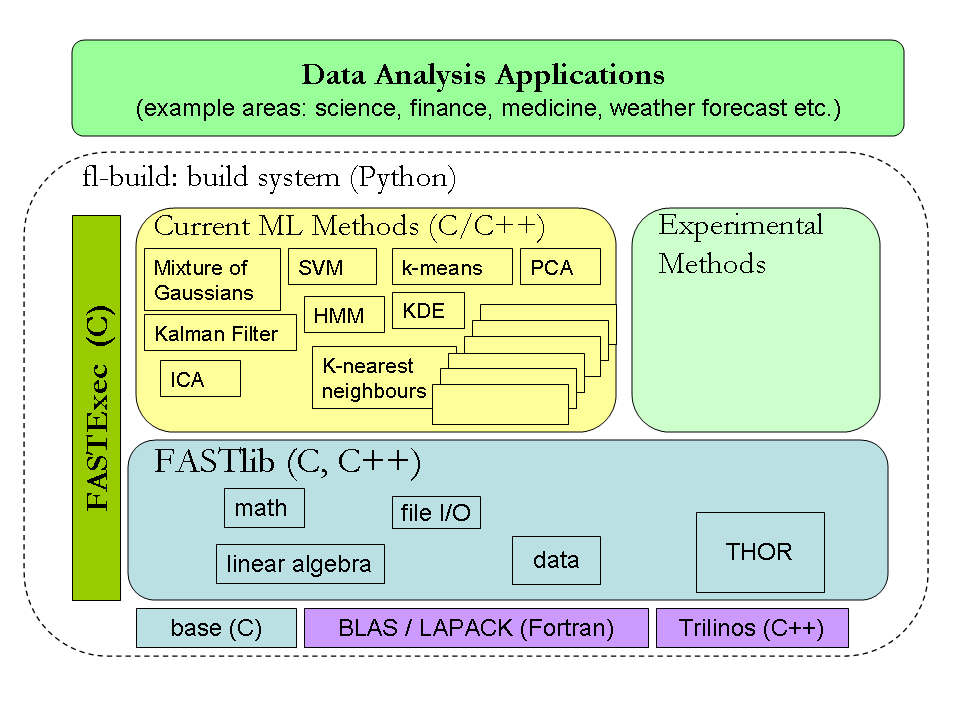
\includegraphics[width=5in]{Fastlib_Archi.png}
\vspace{-0.4in}
\caption{ Overall Organization of the different components of FASTlib}
\label{fastlib_archi}
\end{center}
\end{figure*}

\chapter {Obtaining and Using FASTlib}

FASTlib is intended to be multi-platform, though (without extension)
it relies heavily on the command line; much of the below assumes a
Linux-like interface.  We have tested compilation on the following
systems:
\begin{itemize}
\item Linux: 32-bit x86, 64-bit x86, and Itanium
\item Cygwin (x86 Windows)
\item MacOSX
\end {itemize} 
In order to build FASTlib, you will need the following tools:
\begin {itemize}
\item gcc, g++, and g77 3.4.6; later versions and gfortran should work
\item python 2.2 or later
\item (optional) doxygen and graphviz's dot, for formatted documentation
\end {itemize}

FASTlib is maintained in a Subversion repository at Georgia Tech, but
presently it is available to others in tar-ball format via request.
Let \verb@$FASTLIBPATH@ be the absolute path (i.e.~starting with
\verb@/@) to the directory where you have extracted FASTlib.  You will
need to add \verb@$FASTLIBPATH/script@ to your \verb@$PATH@
environment variable.  This is accomplished differently for different
shells (type \verb@echo $0@ to find out which you are using):
\begin{itemize}
\item For bash or ksh, add to your \verb@.bashrc@ or \verb@.kshrc@
  file (or \verb@.profile@ if the other is absent):
\begin{verbatim}
  export PATH="$FASTLIBPATH/script:$PATH"
\end{verbatim}
\item For csh or tcsh, add to your \verb@.cshrc@ file:
\begin{verbatim}
  setenv PATH "$FASTLIBPATH/script:""$PATH"
\end{verbatim}
\end{itemize}
You will need to close and reopen your terminal to enact the change.
Type \verb@fl-build@ to confirm things are working; this should print
usage information for FASTlib's build system.  Next, try:
\begin{verbatim}
  cd $FASTLIBPATH/u/example
  fl-build main
  ./main --data=fake.arff
\end{verbatim}
This performs 10-fold cross-validation for $k$-nearest-neighbors.  At
the end of the output, you should see
\verb@/kfold/results/p_correct 1.000@; \verb@fake.arff@ was engineered
to be easy.

\section {Code Organization}
The following summarizes the current code organization of FASTlib

\begin{itemize}

\item Core Library
  \begin{itemize}
  \item \verb@fastlib/@ wraps the rest of the library into one convenient include
    \begin{itemize}
    \item \verb@base/   @- compiler abstractions, debugging, and memory management
    \item \verb@col/    @- templated storage types (dynamic arrays, heaps, etc.)
    \item \verb@data/   @- data set types and utilities
    \item \verb@fx/     @- FASTexec client library for managing parameters, timers, and results
    \item \verb@file/   @- file reading, writing, and tokenization
    \item \verb@la/     @- linear algebra routines (mostly a wrapper for BLAS/LAPACK)
    \item \verb@math/   @- a collection of math utilities, to be extended as needed
    \item \verb@par/    @- rudimentary parallelization utilities
    \item \verb@sparse/ @- sparse linear algebra routines (mostly a wrapper for Trilinos)
      \begin{itemize}
      \item \verb@trilinos/@ - includes needed for Trilinos
      \end{itemize}
    \item \verb@thor/   @- templated, parallelized algorithm for GNPs
    \item \verb@tree/   @- utilities to build and manage $kd$-trees, among others.
    \end{itemize}
  \end{itemize}
\item Toolbox of machine learning methods- this is a growing list and the listing below is incomplete as of this writing.
  \begin{itemize}
  \item \verb@MLPACK/@ 
    \begin{itemize}
      \item \verb@allknn/      @- Dual-tree based Nearest Neigbour classifier
      \item \verb@mog_l2e/     @- Mixture of Guassian using L2E
      \item \verb@mog_em/      @- Mixture of Guassian using EM
      \item \verb@nbc/         @- Naive Bayes Classifier
      \item \verb@svm/         @- Support Vector Machine classifier trained using SMO
      \item \verb@nnsvm/       @- Support Vector Machine with Non-negativity constrained wights
      \item \verb@hmm/         @- Hidden Markov Model
      \item \verb@kalman/      @- Kalman Filter
      \item \verb@infomax_ica/ @- ICA using Infomax method
      \item \verb@fastica/     @- ICA using FastICA algorithm 
      \item more $\cdots$
    \end{itemize}
  \end{itemize}
\item Community-build Code
  \begin {itemize}
  \item \verb@contrib/@ - the user directory, which contains individual developers' directories. 
\end {itemize} 
\item  Other
  \begin {itemize}
  \item \verb@bin/      @- files generated by compilation; \verb@make clean@ deletes this
  \item \verb@bin_keep/ @- compiled binaries that should not be cleaned, such as BLAS/LAPACK
  \item \verb@doc/      @- All documentation, including the Doxygen generated ones are here
  \item \verb@examples/ @- Example code and tutorial(s) for using FASTlib library and MLPACK
  \item \verb@include/  @- Symbolic links to all the header files gathered in one place
  \item \verb@lib/      @- linkable libraries
  \item \verb@script/   @- scripts for compiling code, running experiments, etc.
  \item \verb@util/     @- simple utilities used for routine tasks, like random sampling, format conversion etc.
  \end {itemize}
\end{itemize}

\section{Overview of some tools}
To help you get started with using FASTlib and MLPACK for your applications, we provide a brief summary of THOR and some of the cutting edge methods available in the MLPACK. We are in the process of generating user documentation for the rest of the methods in MLPACK. In the meantime please refer to the README files in the individual MLPACK method folders.

\subsection{THOR (Tree High-Order Reduce) framework}
THOR stands for Tree High-Order Reduce. THOR aims to solve the class of high-order-reduce problems (although currently only second-order reduce problems). Its goal is to handle the set of high-order reduce problems that can be accelerated using trees. THOR requires only very abstract information about the tree algorithm at hand, and it is designed to have a lot of freedom and flexibility in executing it. In extremely simple terms, when given a system of reduce functions to solve, in the form of template classes, THOR executes them. THOR considers a combination of summary statistics, pruning rules, and update rules, and uses these to execute your tree-based algorithm in any expansion pattern. Parallel is just another expansion pattern. THOR parallelizes very effectively by dividing the query tree (you must label one of your trees as a query tree even if it is not a query-reference problem) into smaller trees. It then solves each query subtree with the root of the reference tree, which in practice seems to have minimal noticeable overhead compared to solving the problem monolithically. Solving queries independently prevents the need of having to relay pruning information among processors. 

Currently, the software implements a depth-first solver and KD-trees, with data and tree-building occurring on the originating machine. It currently sports excellent multithreaded performance for every problem tested. The networked version has good to excellent performance for small clusters (64 processors) depending on how computationally intensive the problem is. Kernel density estimation, two-point correlation, affinity propagation, high-dimensional nearest neighbors, and more will be able to take advantage of more machines you throw at it. 

Please see \cite{boyer2007tho} for more details on THOR.

\subsection{Kernel Density Estimator}
Kernel density estimation (KDE) is the most widely used and studied nonparametric density estimation method. The 'model' is the reference dataset $\mathcal{R}$ itself, containing the {\it reference points}
indexed by natural numbered. In addition, assume a local kernel function $K_h(\cdot)$ centered upon each reference point, and its scale parameter $h$ (the 'bandwidth'). The common choices for $K_h(\cdot)$ include the spherical, Gaussian and Epanechnikov kernels. We are given the {\it query dataset} $\mathcal{Q}$, which contains {\it query points} whose densities we want to predict.

For the first time, this package offers the following five variants of
the algorithms for efficiently computing kernel density estimates. All
of these algorithms are implemented in C++, adhering to the strict
FastLib standards.

\begin{enumerate}
\item{Dual-tree Fast Gauss Transform with $O(D^p)$ expansion for the
Gaussian kernel~\cite{LEE06}: \verb@kde.h@}
\item{Dual-tree Fast Gauss Transform with $O(p^D)$ expansion for the
Gaussian kernel~\cite{LEE05}: \verb@kde.h@}
\item{The original fast Gauss transform~\cite{ggstrain}: \verb@fgt_kde.h@}
\item{The original improved fast Gauss transform with automatic
parameter tuning~\cite{YANG03}: \verb@original_ifgt.h@}
\item{The KDE algorithm using the multidimensional fast Fourier
transform~\cite{wand94}: \verb@fft_kde.h@}
\end{enumerate}

These algorithms are fairly simple to use. Each algorithm has a
separate build-rule.
\subsubsection{Dual-tree FGT}
In order to compile this tool, do: 
\begin{verbatim}
fl-build kde_bin --mode=fast
\end{verbatim}

In order to run this method, type the following (which consists of
both required and optional arguments) in a single command line:
\begin{verbatim}
./kde_bin} --data=name_of_the_reference_dataset --query=name_of_the_query_dataset
           --kde/bandwidth=0.0130619 --kde/scaling=range --kde/fast_kde_output=fast_kde_output.txt
           --kde/naive_kde_output=naive_kde_output.txt --kde/do_naive --kde/relative_error=0.1
           --kde/multiplicative_expansion
\end{verbatim}

Explanations for the arguments listed with possible values:

\begin{enumerate}
\item{data (required): the name of the reference dataset}
\item{query (optional): the name of the query dataset (if missing, the
 query dataset is assumed to be the same as the reference dataset)}
\item{kde/bandwidth (required): smoothing parameter used for KDE; this
 has to be positive.}
\item{kde/scaling (optional): whether to prescale the dataset - range:
scales both the query and the reference sets to be within the unit
hypercube $[0, 1]^D$ where $D$ is the dimensionality.  - none: default
value; no scaling}
\item{kde/do\_naive (optional): run the naive algorithm after the fast
algorithm.}
\item{kde/fast\_kde\_output (optional): if this flag is present, the
approximated density estimates are output to the filename provided
after it.}
\item{kde/naive\_kde\_output (optional): if this flag is present, the
 exact density estimates computed by the naive algorithm are output to
 the filename provided after it. This flag is not ignored if
 --kde/do\_naive flag is not present.}
\item{kde/relative\_error (optional): relative error criterion for the
 fast algorithm; default value is 0.1 (0.1 relative error for all
 query density estimates)}
\item{kde/multiplicative\_expansion (optional): if present, the KDE
algorithm does $O(p^D)$ expansion for the Gaussian kernel. Otherwise,
it defaults to the $O(D^p)$ expansion.}
\end{enumerate}

\subsubsection{Original Fast Gauss Transform}
In order to compile this part, do: 
\begin{verbatim}
fl-build fgt\_kde\_bin --mode=fast
\end{verbatim}

 To run the FGT-based KDE algorithm, type the
following (which consists of both required and optional arguments) in
a single command line:
\begin{verbatim}
& \mathit{./fgt\_kde\_bin} \
\mathit{--data=name\_of\_the\_reference\_dataset}\\ &
\mathit{--query=name\_of\_the\_query\_dataset} \
\mathit{--kde/bandwidth=0.0130619} \\ & \mathit{--kde/scaling=range} \
\mathit{--kde/fgt\_kde\_output=fgt\_kde\_output.txt}\\ &
\mathit{--kde/naive\_kde\_output=naive\_kde\_output.txt} \
\mathit{--kde/do\_naive}\\ & \mathit{--kde/absolute\_error=0.1}
\end{verbatim}

Explanations for the arguments listed with possible values:

\begin{enumerate}
\item{data (required): the name of the reference dataset}
\item{query (optional): the name of the query dataset (if missing, the
 query dataset is assumed to be the same as the reference dataset)}
\item{kde/bandwidth (required): smoothing parameter used for KDE; this
 has to be positive.}
\item{kde/scaling (optional): whether to prescale the dataset - range:
scales both the query and the reference sets to be within the unit
hypercube $[0, 1]^D$ where $D$ is the dimensionality.  - none: default
value; no scaling}
\item{kde/do\_naive (optional): run the naive algorithm after the fast
algorithm.}
\item{kde/fgt\_kde\_output (optional): if this flag is present, the
approximated density estimates are output to the filename provided
after it.}
\item{kde/naive\_kde\_output (optional): if this flag is present, the
 exact density estimates computed by the naive algorithm are output to
 the filename provided after it. This flag is not ignored if
 --kde/do\_naive flag is not present.}
\item{kde/absolute\_error (optional): absolute error criterion for the
 fast algorithm; default value is 0.1 (0.1 absolute error for all
 query density estimates)}
\end{enumerate}

\subsubsection{Improved Fast Gauss Transform}
In order to compile this algorithm, do: 
\begin{verbatim}
fl-build original\_ifgt\_bin --mode=fast
\end{verbatim}

For the IFGT-based KDE algorithm, type the
following (which consists of both required and optional arguments) in
a single command line:
\begin{verbatim}
& \mathit{./orignal\_ifgt\_bin} \
\mathit{--data=name\_of\_the\_reference\_dataset}\\ &
\mathit{--query=name\_of\_the\_query\_dataset} \
\mathit{--kde/bandwidth=0.0130619} \\ & \mathit{--kde/scaling=range} \
\mathit{--kde/ifgt\_kde\_output=ifgt\_kde\_output.txt}\\ &
\mathit{--kde/naive\_kde\_output=naive\_kde\_output.txt} \
\mathit{--kde/do\_naive}\\ & \mathit{--kde/absolute\_error=0.1}
\end{verbatim}

Explanations for the arguments listed with possible values:

\begin{enumerate}
\item{data (required): the name of the reference dataset}
\item{query (optional): the name of the query dataset (if missing, the
 query dataset is assumed to be the same as the reference dataset)}
\item{kde/bandwidth (required): smoothing parameter used for KDE; this
 has to be positive.}
\item{kde/scaling (optional): whether to prescale the dataset - range:
scales both the query and the reference sets to be within the unit
hypercube $[0, 1]^D$ where $D$ is the dimensionality.  - none: default
value; no scaling}
\item{kde/do\_naive (optional): run the naive algorithm after the fast
algorithm.}
\item{kde/ifgt\_kde\_output (optional): if this flag is present, the
approximated density estimates are output to the filename provided
after it.}
\item{kde/naive\_kde\_output (optional): if this flag is present, the
 exact density estimates computed by the naive algorithm are output to
 the filename provided after it. This flag is not ignored if
 --kde/do\_naive flag is not present.}
\item{kde/absolute\_error (optional): absolute error criterion for the
 fast algorithm; default value is 0.1 (0.1 absolute error for all
 query density estimates)}
\end{enumerate}

\subsubsection{FFT-based KDE}
In order to compile this code, do: 
\begin{verbatim}
fl-build fft\_kde\_bin --mode=fast
\end{verbatim}
For the FFT-based KDE algorithm, type the
following (which consists of both required and optional arguments) in
a single command line:
\begin{verbatim}
& \mathit{./fft\_kde\_bin} \
\mathit{--data=name\_of\_the\_reference\_dataset}\\ &
\mathit{--query=name\_of\_the\_query\_dataset} \
\mathit{--kde/bandwidth=0.0130619} \\ & \mathit{--kde/scaling=range} \
\mathit{--kde/fft\_kde\_output=fft\_kde\_output.txt}\\ &
\mathit{--kde/naive\_kde\_output=naive\_kde\_output.txt} \
\mathit{--kde/do\_naive}\\ & \mathit{--kde/num\_grid\_pts\_per\_dim=128}
\end{verbatim}

Explanations for the arguments listed with possible values:

\begin{enumerate}
\item{data (required): the name of the reference dataset}
\item{query (optional): the name of the query dataset (if missing, the
 query dataset is assumed to be the same as the reference dataset)}
\item{kde/bandwidth (required): smoothing parameter used for KDE; this
 has to be positive.}
\item{kde/scaling (optional): whether to prescale the dataset - range:
scales both the query and the reference sets to be within the unit
hypercube $[0, 1]^D$ where $D$ is the dimensionality.  - none: default
value; no scaling}
\item{kde/do\_naive (optional): run the naive algorithm after the fast
algorithm.}
\item{kde/fft\_kde\_output (optional): if this flag is present, the
approximated density estimates are output to the filename provided
after it.}
\item{kde/naive\_kde\_output (optional): if this flag is present, the
 exact density estimates computed by the naive algorithm are output to
 the filename provided after it. This flag is not ignored if
 --kde/do\_naive flag is not present.}
\item{kde/num\_grid\_pts\_per\_dim (optional): specifies the number of
grid points per each dimension (for discretizing and gridding the
datasets). This is the only way to do any type of error control on
approximated KDE values. In general, the higher the value, more
accurate the density estimates will be. The default value is 128.}
\end{enumerate}

\subsection{Orthogonal Range Search}
The orthogonal range search problem answers the following question:
Given a set of points $\mathcal{R}$ in $D$-dimensional Euclidean
space, what points lie in the search window: $[l(1), u(1)]\times
[l(2),u(2)]\times \cdots \times [l(D),u(D)]$?

\subsubsection{FastLib-based Orthogonal Range Search}
This package offers two algorithms - a naive algorithm and a
tree-based algorithm for computing orthogonal range search. All of
these algorithms are implemented in C++, adhering to the strict
FastLib standards.

In order to compile this package, do: 
\begin{verbatim}
fl-build ortho\_range\_search\_bin --mode=fast
\end{verbatim}
In order to run this tool, type the following (which consists of
both required and optional arguments) in a single command line:
\begin{verbatim}
& \mathit{./ortho\_range\_search\_bin} \ \mathit{--data=dataset} \
\mathit{--do\_naive}
\end{verbatim}

Explanations for the arguments listed with possible values:

\begin{enumerate}
\item{data (required): the name of the reference dataset}
\item{do\_naive (optional): run the naive algorithm after the fast
algorithm.}
\end{enumerate}
The example code usages are described in ortho\_range\_search.h.

\subsection{EMST}
The FASTlib EMST code implements a dual-tree version of Bor\r{u}vka's algorithm for finding minimum spanning trees.  Bor\r{u}vka's algorithm is similar to Kruskal's well-known algorithm.  Instead of connecting the two closest components of the spanning forest, Bor\r{u}vka's algorithm connects each component to its nearest neighbor.  We accelerate the computation of these neighbors in each step using a dual-tree search.  

\textbf{Please note:}  This algorithm is awaiting publication.  It is not intended for widespread distribution.  

\vspace{0.2in}
\noindent \textbf{Command line use.}  
\begin{itemize}
\item \textbf{Compile:} \texttt{fl-build emst\_main}
\item \textbf{Run:} \texttt{./emst\_main --data=filename}  This will create a file ``output.txt'' with the minimum spanning tree in edge-list form.
\item \textbf{Command-line parameters:}
  \begin{itemize}
  \item \texttt{string --data} : The name of the input file
  \item \texttt{int --dtb/leaf\_size} : Number of points in the leaves of the tree.  \emph{Default}=\texttt{1}
  \item \texttt{bool --do\_naive} : If true, will perform both the \textsc{DualTreeBoruvka} algorithm and a naive implementation of Bor\r{u}vka's algorithm and will compare the results.
  \item \texttt{string --naive/output\_filename} : The name of the file where the edge list of the naive computation will be printed.  \emph{Default}=\texttt{naive\_output.txt}
  \item \texttt{string --dtb/output\_filename} : The name of the file where the edge list from \textsc{DualTreeBoruvka} will be printed.  \emph{Default}=\texttt{output.txt}
  \end{itemize}
\end{itemize}

\begin{figure}[ht]
\fbox{
\begin{minipage}[t]{0.95\linewidth}
\spcA \textbf{function} boruvka($V$) \newline
\spcB $E = \emptyset$ \newline
\spcB \textbf{while} $|E| < |V| - 1$ \newline
\spcC \textbf{for} all components $C$ \newline
\spcD $(u, v) = \arg \min d(i, j)$ where $i \in C, j \not\in C$\newline
\spcD $E = E \cup (u, v)$ \newline
\spcB \textbf{return} $E$
\end{minipage}
}
\vspace{-0.1in}
\caption{Pseudocode for Bor\r{u}vka's algorithm.}
\label{boruvka_pseudocode}
\end{figure}

\vspace{-1.5in}

\begin{figure}[tbh]
\fbox{
\begin{minipage}[t]{0.95\linewidth}
\spcA \textbf{init} $E = \emptyset$  \newline
\spcA \textbf{function} dtb($Q^{\textrm{root}}, R^{\textrm{root}}$) \newline
\spcB \textbf{while} $|E| < |V| - 1$ \newline
\spcC $\forall Q, a^u(Q) = \infty, \forall q, a(q) = \infty$ \newline
\spcC cnn($Q^{\textrm{root}}, R^{\textrm{root}}$) \newline
\spcC for all $q$, $E = E \cup n(q)$ \newline
\spcB \textbf{end}\newline
\spcB \textbf{return} $E$ \newline
\newline
\spcA \textbf{function} cnn($Q, R$) \newline
\spcB \textbf{if} $a^u(Q) < d^l(Q, R)$, \textbf{return} \newline
\spcB \textbf{else if} $Q$ and $R$ are fully connected, \textbf{return} \newline
\spcB \textbf{else if} $(Q, R) = (\{q\}, \{r\})$ \newline
\spcC \textbf{if} $d(q, r) < a(q)$ \newline
\spcD $a(q) = d(q, r), n(q) = r$ \newline
\spcD \textbf{if} $a(q) < a^u(Q)$ \newline
\spcE $a^u(Q) = a(q)$ \newline
\spcB \textbf{else} \newline
\spcC prioritize $\{R^1, R^2\} = \{R^L, R^R\}$ by $d^l(Q^L, \cdot)$ \newline
\spcD cnn($Q^L, R^1$), cnn($Q^L, R^2$) \newline
\spcC prioritize $\{R^1, R^2\} = \{R^L, R^R\}$ by $d^l(Q^R, \cdot)$ \newline
\spcD cnn($Q^R, R^1$), cnn($Q^R, R^2$) \newline
\spcC $a^u(Q) = \max\{a^u(Q^L), a^u(Q^R)\}$
\end{minipage}
}
\caption{Pseudocode for our \textsc{DualTreeBoruvka} algorithm.  $a^u(Q)$ represents the upper bound on candidate neighbors found so far for node $Q$, and $d^l(Q, R)$ represents the minimum distance between the bounding boxes of $Q$ and $R$.  $n(q)$ is the current candidate for the nearest neighbor of $q$, and $a(q) = d(q, n(q))$.}
\label{DTB}
\end{figure}


\chapter {Code development using FASTlib}
 
This chapter provides a very brief tutorial of modifying build files, using FASTexec and inbuilt debugging tools etc. to help you get started with writing your own code using FASTlib. For more extensive tutorial please refer to the FASTlib developer tutorial and API reference manual.

\section {Using the build tool}

As stated earlier, building is done via the fl-build tool, which stands for FASTlib build. This tool reads through very short files which just have a list of sources (.cc files), headers (.h files), and other sub-packages it depends on, and produces a Makefile, which it runs automatically.

There are a handful of compilation modes supported by fl-build, specified by the \verb = --mode=mode = parameter. Each mode has a use, and enables certain flags:
\begin{itemize}
\item verbose: tracking the execution of a program when it's infeasible to step through manually. disables optimizations, enables printing of verbosity messages
\item debug: allow best use with gdb for tracking bugs. disables optimization, enables all debug checks, enables highest level of gdb.
\item check (default mode): regular development. enables code optimizations and leaves in debug checks, at a 25% or so penalty. gdb symbols are compiled in but may be inaccurate due to optimizations.
\item fast: timing runs, for the fairest timing comparisons. debug symbols still enabled but may be inaccurate.
\item unsafe: optimizations that might alter correctness, and often will slow the program down.
\item profile: speed profiling. compile with --mode=profile, run your program, and run gprof ./binaryfile | less to see what the bottleneck is. 
\end{itemize}
The command line flags are listed in script/buildsys.py. 

Thus, we could re-build the example, but turn off all debug checks:
\begin{verbatim}
fl-build main --mode=debug
\end{verbatim}
To add custom flags, add \verb@--cflags@. To get increased performance on Pentium 4 and define a macro called \verb@COAGULATE@, you would use:
\begin{verbatim}
fl-build mybinary --mode=fast --cflags="-march=pentium4 -DCOAGULATE"
\end{verbatim}


\subsection{Writing build files}

The fl-build tool looks in the current directory for a file called build.py. The build file is executed as straight Python code, with access to a few specific functions defined by the build system, that correspond to ``meta build rules''. In processing these, the build system recursively pulls build files from other directories and resolves the dependencies. A Makefile is then created in your current directory, which fl-build automatically runs for you.

Here is a sample build rule that will build an executable test compiled from test.cc and test.h, and link it against the fastlib front-end library:
\begin{verbatim}
binrule(
   name = "test",
   sources = ["test.cc"],
   headers = ["test.h"],
   linkables = ["fastlib:fastlib"]
   )
\end{verbatim}
Each string you see is actually processed by the build system, which figures out what you are referring to. If there is no colon ``:'' character, it looks for a file in the same directory as the build file. If it finds a ``:'', such as ``fastlib:fastlib'', it looks in the directory ``fastlib'' for a rule named ``fastlib'' -- the left part of the colon is the directory, the right part is the rule name. For example, the full path to the rule for the main executable in \verb@example@ would be \verb@"example:main"@.

Next, suppose you want to create a small reusable library. Taking a look at the build file \verb@u/example/build.py@,
\begin{verbatim}
librule(
    name = "example",              # this line can be safely omitted
          # (since this is u/example, the build system
          # will automatically name it "example" if you omit it -- most
          # other sub-packages will omit the name)
    sources = ["helper.cc"],       # files that must be compiled
    headers = ["helper.h"],        # include files part of the 'lib'
    deplibs = ["fastlib:fastlib"]  # depends on fastlib core
    )

binrule(
    name = "main",                 # the executable name
    sources = ["main.cc"],         # compile main.cc
    headers = [],                  # no extra headers
    linkables = [":example"]       # depends on example in this folder
    )
\end{verbatim}

\section{Use of C++}

FASTlib is C++, but only to an extent. If you are familiar with C, you will have no problem. The things we use from C++ is:
\begin{itemize}
\item Templates, for pluggability (used very extensively in THOR)
\item Classes, for coupling data and operations over the data
\item Destructors, to avoid unnecessary clean-up code, and to better support templates 
\end{itemize}
FASTlib mostly avoids inheritance, virtual functions, and operator overloading. It also notably avoids most constructors due to their pickiness about when they are called. Here's an example of what this looks like. In particular, we'll create a multiplication table:
\begin{verbatim}
Matrix mult_table;

mult_table.Init(10, 10); // make it 10 rows by 10 columns

for (index_t i = 0; i < 10; i++) {
  for (index_t j = 0; j < 10; j++) {
    mult_table.set(i, j, i * j);
  }
}
// the matrix does not have to be freed
\end{verbatim}
Some quick notes before we move on. The matrix must be initialized before it is usable, but keep in mind everything is freed by default. Caution -- if you declare a matrix and never initialize it, the program will crash at the end of the function. In debug mode, many FASTlib classes will let you know that this is happening.  We are assessing this behavior and future versions of FASTlib may instead gurantee safe destruction if it doesn't critically impact performance.  (The \verb@index_t@ type is usually an regular int, but is wired through the system to become 64-bit if you tell it to.)

\section{Copying and Aliasing}

C++ is infamous for its desire to make copies of everything. If you forget to pass a parameter as a constant reference (\verb@const ClassName \&@), the copy constructor is called automatically and any sane copy constructor must make a completely new and distinct instance of the object.  The cannonical means of preventing this behavior is to define the copy constructor (and assignment operator) as private.  This will result in compilation errors in lieu of mysteriously slow or buggy.  We provide a macro to automate this process:
\begin{verbatim}
class X {
  FORBID_ACCIDENTAL_COPIES(X);
 public:
  ...
}
\end{verbatim}
Sometimes, though, you really need to make copies, or at least things like copies. Many classes, especially pure-data classes, do have functional copy constructors, and yet others support a Copy method to explicitly perform the task of copy construction.  They Copy method operates as if it were an Init function.

The Vector and Matrix classes also support a concept of aliasing. A vector can be responsible for its own memory, or it could point to some column within a matrix; a matrix can also refer to a subset of another matrix's columns. The concept is simple, but there is one caveat: without garbage collection, somebody eventually has to free the memory. Each Vector and Matrix then knows whether it is the owner of the memory it points to, and if it is, it will free the data automatically; otherwise, it is only an alias.

An example is shown here:
\begin{verbatim}
   Matrix original;
   original.Init(5, 5);
   ...
   for (int j = 0; j < 3; ++) {
     Matrix weak_alias;
     weak_alias.Alias(original); // this matrix now aliases the original
     weak_alias.set(j, j, 999.0); // this modifies the original matrix
     // the destructor of weak_alias is called, but the memory is not freed
   }
   Matrix newowner;
   newowner.Own(&original); // newowner
   Matrix copy;
   copy.Copy(original); // a completely new copy 
   original.Destruct(); // newowner is still valid
   original.Init(99, 99);
\end{verbatim}

\section{Debugging}

C++, and equally C, can sometimes make it easy to shoot yourself in the foot. To help you avoid this, we made debugging an important part of FASTlib.

The build system by default will enable all checks in the form of \verb@#ifdef DEBUG@ (we'll get back to this later). These checks and safeguards, such as bounds checking and memory poisoning, are present in nearly all core FASTlib classes. If you are debugging and find \verb@0xDEADBEEF@ or \verb@2146666666 == 0x7FF388AA == NaN@, it probably means you forgot to initialize something; if you go beyond the end of a Vector, it will let you know. In practice, these have a 20% or so performance penalty -- as a habit, we've found it's just fine to leave these on until you want to run timing experiments. In machine learning code, since you can sometimes generate seemingly good results from garbage data, these types of safeguards are almost essential.

To use debugging yourself, plaster your code with the following:
\begin{itemize}
\item \verb@DEBUG_ASSERT_MSG(condition, format, ...)@ - If the condition is false, your program will print the formatted message to stderr and die.
\item \verb@VERBOSE_GOT_HERE(3)@ - If verbosity is greater than 3 and verbose-mode is compiled on, it will print the function and line number. 
\end{itemize}
You can safely leave these in at no cost in non debug mode. To set verbosity level to 3.0, you would specify the command line argument: \verb@--debug/verbosity_level=3.0@.See the Doxygen for \verb@base/debug.h@ for more information.

\section{FASTexec - Command-line parameters and experimentation}

We felt it is important that machine learning researchers can run a lot of experiments without too much trouble. Parameter passing is integral to the experimentation process, so we unified these.

The core idea behind the system is that within one run of your program, a hierarchial data store is created. In some ways it is similar to a ``Windows registry'' except it only has a very brief existence. In fact, it more like an XML document tree, except without attributes, and has a ``stateless'' output format.

\subsubsection{Basic command-line parameters}

Let's look at a non-trivial example. We're measuring how different strided memory access patterns affect cache performance (something you probably won't care about, but is trivial to code):
\begin{verbatim}
#include "fastlib/fastlib.h"
int main(int argc, char *argv[]) {
  fx_init(argc, argv); // initialize command-line parameters and the data store
  int count = fx_param_int_req( // get a REQUIRED integer parameter
      NULL, // directly from command line (not from a sub module)
      "count"); // called "count", as in --count=num
  int stride = fx_param_int(NULL, "stride", 1); // defaults to stride 1
  double factor = fx_param_double(NULL, "factor", 1.0); // default value 1.0
  
  ArrayList<double> values;
  values.Init(count);

  fx_timer_start(NULL, "strides"); // timers have names
  // Let's see how stride affects cache performance
  for (int s = 0; s < stride; s++) {
    for (int j = s; j < count; j += stride) {
      values[j] = factor * j;
    }
  }
  fx_timer_stop(NULL, "strides");
  fx_format_result(NULL, "success", "%d", 1); // store some result
  fx_done();
}
\end{verbatim}

The useful functions we used were \verb@fx_param_int@ (to get an integer), \verb@fx_param_double@ (to get a double-precision value), \verb@fx_timer_{start|stop}@ to have timers, and \verb@fx_done()@ to output the results. I ran this example with the parameters:
\begin{verbatim}
./test --count=10000 --factor=2.0
\end{verbatim}
and the following text resulted:
\begin{verbatim}
<code>
/timers/strides/children/sys 0.000000
/timers/strides/children/user 0.000000
/timers/strides/self/sys 0.000000
/timers/strides/self/user 0.000000
/timers/strides/wall/sec 0.000061
/timers/default/children/sys 0.000000
/timers/default/children/user 0.000000
/timers/default/self/sys 0.000000
/timers/default/self/user 0.000000
/timers/default/wall/sec 0.000354
/params/stride 1
/params/fx/timing 0
/params/debug/print_notify_headers 1
/params/debug/pause_on_nonfatal 0
/params/debug/abort_on_nonfatal 0
/params/debug/print_warnings 1
/params/debug/print_got_heres 1
/params/debug/verbosity_level 1
/params/factor 2.0
/params/count 10000
/results/success 1
/info/rusage/children/nivcsw 0
/info/rusage/children/nvcsw 0
/info/rusage/children/nsignals 0
/info/rusage/children/msgrcv 0
/info/rusage/children/msgsnd 0
/info/rusage/children/oublock 0
/info/rusage/children/inblock 0
/info/rusage/children/nswap 0
/info/rusage/children/isrss 0
/info/rusage/children/idrss 0
/info/rusage/children/ixrss 0
/info/rusage/children/maxrss 0
/info/rusage/children/majflt 0
/info/rusage/children/minflt 0
/info/rusage/children/stime 0.000000
/info/rusage/children/utime 0.000000
/info/rusage/children/WARNING your_OS_might_not_support_all_of_these
/info/rusage/self/nivcsw 1
/info/rusage/self/nvcsw 3
/info/rusage/self/nsignals 0
/info/rusage/self/msgrcv 0
/info/rusage/self/msgsnd 0
/info/rusage/self/oublock 0
/info/rusage/self/inblock 0
/info/rusage/self/nswap 0
/info/rusage/self/isrss 0
/info/rusage/self/idrss 0
/info/rusage/self/ixrss 0
/info/rusage/self/maxrss 0
/info/rusage/self/majflt 0
/info/rusage/self/minflt 393
/info/rusage/self/stime 0.002999
/info/rusage/self/utime 0.002999
/info/rusage/self/WARNING your_OS_might_not_support_all_of_these
/info/system/kernel/build %231%20SMP%20Tue%20Jan%2023%2012%3A49%3A51%20EST%202007
/info/system/kernel/release 2.6.9-42.0.8.ELsmp
/info/system/kernel/name Linux
/info/system/arch/name x86_64
/info/system/node/name shannon.cc.gatech.edu
\end{verbatim}
We admit this is a lot of text, but when you later comb through the results, you can select only the portions you care about. Briefly, each portion of the tree:
\begin{itemize}
\item params/ - Parameters you were called with. Default parameters are explicitly stored in case you later change what the default values are.
\item timers/ - Each timer. There will always be a default timer, which runs between \verb@fx_init@ and \verb@fx_done@.
\item results/ - Results that you decided to emit.
\item info/rusage/ - System information related to rusage. See the manpage for getrusage(2).
\item info/system/ - Information on the system run on. See manpage for uname(2). 
\end{itemize}
This output could indeed just be an s-expression, or it could be an attribute-less XML file. We chose this path-value dump format because it is stateless -- i.e. anyone can process it with a little bit of grep. Corruption in the file will only affect it until the next newline.

\subsection{Running automated experiments and collecting results}

Running experiments and collecting results is made simpler using FASTexec. After using the FASTexec code to store output variables in the datastore, you can use FASTexec to run multiple experiments. If you type the command:
\begin{verbatim}
fx-run | less
\end{verbatim}
you will see the help screen for fx-run. This program will run your executable with all combinations of the parameters you give it, and save results in a directory called fx that is created in the same directory you run the tests. After that, gather results using fx-csv to make an Excel-compatible comma-separated-values file, or fx-latex to create a properly escaped LaTeX table.

You can try an example with the K-nearest-neighbors classifier example in u/example:
\begin{verbatim}
  cd $FASTLIBPATH/u/example && fl-build main
  fx-run knn_k ./main --knn/k=1,2,3,4,5 --data=../../../../fake.arff
  fx-csv knn_k ./main /params/knn/k /kfold/results/p_correct
  fx-latex knn_k ./main /params/knn/k /kfold/results/p_correct --preview
\end{verbatim}

\section{Some tips}

\subsection{Success and failure}

The \verb@success_t type@ in \verb@base/common.h@ defines our standard for indicating success or failure. Rather than assuming 1 or 0 or -1 indicates something or other, we explicitly return \verb@SUCCESS_PASS@ (succeeded), \verb@SUCCESS_FAIL@ (failed), or \verb@SUCCESS_WARN@ (something was suboptimal).

\subsection{Basic types}

You will notice heavy use of \verb@index_t@ (in \verb@base/scale.h@) rather than integers. For practical purposes, \verb@index_t@ is a signed integer -- signed so you can loop over >= 0. On 32-bit and 64-bit Intel/AMD machines, this will be 32-bits, which is the fastest int for both systems and is relatively compact. But if you want to operate on datasets larger than a few gigabytes, you can define the \verb@SCALE_LARGE@ macro, and these will instantly switch to the largest size your computer can address.

Also, the \verb@base/basic_types.h@ file (it will be in bin/ since it is auto-generated) defines standard int16, int32, int64, uint16, uint32, uint64 types.

\subsection{Printf versus Streams}

We operate under the assumption that more of our audience is familiar with C I/O than with C++ I/O, especially when it comes to fancy floating-point formatting. The caveat is that printf only works with native types like int, short, long. To print an \verb@index_t@, you use:
\begin{verbatim}
printf("Iteration %"LI"d complete.", some_index_var);   // no special formatting
printf("Iteration %04"LI"d complete.", some_index_var); // with formatting
\end{verbatim}
The LI macro is a string that will have the suitable ``l'' modifier for \verb@index_t@ (see man sprintf for more details). For other types:
\begin {itemize}
\item int16 and uint16: L16
\item int32 and uint32: L32
\item int64 and uint64: L64 
\end{itemize}
Alternately, you can just cast the variable to a native type like (int) (short) or (long), if you want to be lazy.

\chapter {Beyond this Document} 

FASTlib has a growing body of documentation. We have an online documentation of all the supported classes and API (currently temporarily available at http://www.cc.gatech.edu/\~nadeem/fastlib). There is also a code walkthrough tutorial that shows how to implement a simple machine learning method (k-NN) starting from scratch. A cook-book with tutorial and code snippets for doing various common tasks is also available. We will bringing these together through a web-page to support FASTlib.

\bibliographystyle{plain}
\bibliography{fastlib}
\end{document}
